% !TEX root = 0_main.tex
\chapter{Evaluation}
We use a variety of benchmark functions to evaluate the performance and practicability of TinyGarble.
In this section, we first describe our experimental setup (\sect{sect:exp}) and metrics for quantifying the performance of TinyGarble (\sect{ssect:metrics}).
We outline the performance comparison of TinyGarble (with HDL synthesizer and our custom libraries) on combinational benchmark functions with PCF \cite{kreuter2013pcf}, one of the best known earlier automated methodologies to generate circuits for garbling in \sect{ssect:customlib}.
TinyGarble's performance in generating sequential circuits for benchmark functions using a standard HDL synthesis tool is demonstrated in \sect{ssect:seqeval}.
\sect{ssect:cacheTime} shows the CPU time for various numbers of sequential cycles which demonstrates the effect of memory footprint reduction in garbling time.
\sect{ssect:HLSeval} shows a comparison between TinyGarble's performance using an HLS tool (input written in C) and using a conventional HDL synthesis tool (input given in Verilog).
Lastly, \sect{ssect:mipsres} shows the result of our garbled processor and implementation of Hamming distance as a benchmark.

We also compare the performance of the commercial logic synthesis tool with the academic, open-source tools in Appendix \ref{app:seqos}.
We show that in most cases, the performance of the open-source tool is comparable to the commercial tool.

\section{Experimental Setup}
The circuit generations are all done on a system with Linux RedHat Server 5.6, 8~GB of memory, and Intel Xeon X5450 CPU @ 3~GHz.
We use another system with Ubuntu 14.10 Desktop, 12.0~GB of memory, and Intel Core i7-2600 CPU @ 3.4GHz to assess the timing performance of the sequential garbling scheme in \sect{ssect:cacheTime}.

Two sets of HDL synthesis tool chains are used in our experiments: one commercial and one open-source (Appendix \ref{app:seqos}).
Our commercial HDL level synthesis tool is Synopsis Design Compiler (DC) 2010.03-SP4 \cite{tool:DesignCompiler}.
We also use the Synopsis Library Compiler from the DC package to interpret our custom technology library.
In \sect{ssect:HLSeval}, we utilize Xilinx Vivado HLS \cite{tool:Vivado}, a commercially available HLS tool whose inputs are written in the C/C++ programming language.
We emphasize that TinyGarble can operate with any commercial or open-source sequential HDL-level (or HLS) synthesizer, as long as the synthesizer is capable of performing state-of-the-art logic optimization and mapping algorithms.

\section{Performance Metrics}
We use the following metrics to measure the efficiency of TinyGarble for generating garbled circuits:

\begin{itemize}
\item
	\textit{Memory Footprint Efficiency} ($\mathit{MFE}$): $$\mathit{MFE} = \dfrac{q_{0}}{q},$$ where $q_{0}$ is the total number of gates in the reference circuit and $q$ is the total number of gates in the circuit under evaluation.
	The maximum number of tokens that need to be stored at any point during garbling/evaluation as well as memory required for storing circuit description is directly proportional to the number of gates in both sequential and combinational circuits.
	Thus, the total number of gates is approximately proportional to the memory footprint.

\item
	\textit{Number of Garbled Tables} ($\mathit{\#GT}$): $$\mathit{\#GT} = \#nonXOR\times c,$$ where $\#nonXOR$ is the number of non-XOR gates in a circuit and $c$ is the number of sequential cycles that the circuit needs to be garbled/evaluated.
	In free XOR-based GC schemes, each non-XOR gate requires a garbled table to be generated by the garbler and sent to the evaluator at each sequential cycle.
	Thus, this metric is an estimate of both the computation and communication time.

\item
	\textit{Garbled Tables Difference} ($\mathit{GTD}$ (\%)): $$\mathit{GTD} = \dfrac{\mathit{\#GT} - \mathit{\#GT}_{0}}{\mathit{\#GT}_{0}} \times 100,$$ where $\mathit{\#GT}_{0}$ is the total number of garbled tables for the reference circuit and $\mathit{\#GT}$ is the total number of garbled tables for the circuit under evaluation.
	When comparing a sequential with a combination circuit, positive $\mathit{GTD}$ shows an \emph{overhead} (caused by folding a circuit with an asymmetric loop, see \sect{sect:sequen}) in total computation and communication time resulting from an excessive number of garbled tables generated in the sequential circuits.
	However, in general, negative $\mathit{GTD}$ shows improvement in the number of non-XOR gates and generated garbled tables that results from logic synthesis optimization.
\end{itemize}

\section{Benchmark functions}
We evaluate TinyGarble's circuit generation method on various benchmark functions.
Several of these functions have been used in previous works, e.g., PCF~\cite{kreuter2013pcf}.
In the following, we introduce our benchmarks and explain how we fold them into a sequential representation.

\textit{Sum.} This function receives two $N$-bit inputs and outputs an $N$-bit sum.
The sum function is implemented in $N$ steps of one bit sums by keeping the carry bit.
Thus, it can be folded up to $N$ times without any significant overhead in number of garbled tables ($\mathit{\#GT}$).

\textit{Hamming Distance.} This function receives two $N$-bit inputs and outputs the $\log_2(N)$-bit Hamming distance between them.
The Hamming distance between two numbers is the number of positions at which the corresponding bits are different.
A possible combinational implementation of the $N$-bit Hamming distance uses a binary tree of adders that sums all $1$-bit values from the bit differences to a final Hamming distance consisting of $\log_2(N)$ bits \cite{boyar2006concrete}.
This implementation cannot be folded easily.
However, we can fold this function into $N$-cycles of one XOR and one $\log_2(N)$-bit adder.
This causes an overhead compared to the combinational circuit.

\textit{Compare (Millionaires problem).} This function receives two $N$-bit unsigned input values and outputs a greater than signal consisting of one bit that indicates if the first input is greater than the second one.
The comparison function can be implemented in $N$ steps of subtraction by keeping the carry bit \cite{kolesnikov2009improved}.
Thus, it can be folded up to $N$ times without any significant overhead.

\textit{Multiplication.} This function receives two unsigned $N$-bit inputs and outputs their unsigned $N$-bit product.
The multiplication function consists of $N$ additions and shifts.
The shift operations result in an asymmetric structure in this function.
Thus, folding it up to $N$ times may increase the overhead.

\textit{Matrix Multiplication.} This function receives two $N\times N$ matrices consisting of $32$-bit unsigned numbers and outputs an $N\times N$ matrix equal to the product of the input matrices.
The $N\times N$ matrix multiplication function consists of three $N$-cycle nested loops with a symmetric structures.
It can be folded up to $N^3$ times without any significant overhead.

\textit{AES-128.} This function receives a 128-bit plaintext and 128-bit round keys and outputs a 128-bit ciphertext based on the Rijndael algorithm.
The AES-128 function consists of 10 rounds with almost symmetric structure.
Ideally, it can be folded up to $10$ times without any significant overhead.

\textit{SHA3.} This function receives $576$-bit inputs and outputs a $1600$-bit number equal to the SHA3 hash of the input.
We implement the Keccak-f permutations[$1600$] procedure for realizing this function.
The SHA3 function consists of 24 steps, each with a symmetric structure.
It can be folded 24 times without any significant overhead.

\section{Combinational Garbled Circuit}
To show the performance gain of using our custom libraries, we compare TinyGarble combinational circuits with circuits reported in PCF \cite{kreuter2013pcf}.
We choose PCF because among the \emph{automated} GC tools available at the time of writing, it shows better results for most of the benchmarks.
In some other work like FastGC \cite{huang2011faster}, a number of benchmark circuits have been more aggressively improved (compared to PCF) using ad-hoc and mostly manual optimizations, but without a generalizable methodology.

The comparison is shown in \tab{table:result-comb}.
We compute the garbled tables difference $\mathit{GTD}$ (see \sect{ssect:metrics}) of various benchmarks by using circuits reported in PCF as reference ($\mathit{GTD}$\textsuperscript{PCF}).
It can be seen that the combinational circuits generated by TinyGarble have non-positive $\mathit{GTD}$\textsuperscript{PCF} which means that the number of garbled tables are less than or equal to that of PCF circuits.
We also compare the memory footprint by computing the memory footprint efficiency $\mathit{MFE}$ with PCF as reference ($\mathit{MFE}$\textsuperscript{PCF}).
We observe that $\mathit{MFE}$\textsuperscript{PCF} is larger than 1 (up to 9.3).
This means that even without using sequential circuits, the memory footprint can be reduced by almost an order of magnitude by using TinyGarble custom libraries and standard HDL synthesis.

In case of Hamming distance, TinyGarble shows, on average, $80\%$ improvement in number of garbled tables.
Another automated tool CBMC-GC \cite{franz2014cbmc} reports better result compared to PCF for Hamming 160 (non-XOR $\numprint{4738}$, total gates $\numprint{20356}$).
However, TinyGarble shows $66\%$ improvement in number of garbled tables compared to CBMC-GC.
In case of 256-bit and 1024-bit Multiplication, and $8\times 8$ and $16\times 16$ Matrix Multiplication, because of the huge (impractical) sizes, Synopsis DC was unable to generate the entire combinational circuit.
This is because Synopsis DC is a tool developed for commercial applications.
The real-life applications are almost always written sequentially, otherwise the design would not be scalable or even amenable to offline compilation onto a hardware circuit.
We emphasize that our sequential circuit ($c>1$) provides the exact same functionality while having a very small memory footprint compared with the reference circuit.

\subsection{Comparison with Hand-Optimized Circuits}
The netlists generated by the automated flow of TinyGarble show similar performance as the hand-optimized netlists in many cases.
For example, \cite{kolesnikov2009improved} describe an $N$-bit sum circuit with $5N$ gates of which $N$ gates are non-XOR and an $N$-bit comparison circuit with $4N$ gates of which $N$ gates are non-XOR.
The circuits generated by TinyGarble have about the same number of gates for these two functions.
Note that one can always add any hand-optimized module to the synthesis library of TinyGarble.

\section{Sequential Garbled Circuit}
As described in \sect{sect:sequen}, the user has the degree of freedom to fold a combinational circuit and convert it to a sequential one to reduce the memory footprint.
$c$ denotes the number of sequential cycles required to garble/evaluate the circuit.
This value demonstrates the amount of folding that is performed before the circuit is input to the synthesizer.
The user defines the value of $c$ and writes her own input function in an HDL or a higher level language such that the function is evaluated in $c$ sequential cycles.

We use Memory Footprint Efficiency ($\mathit{MFE}$), to evaluate the reduction in memory requirement.
We use TinyGarble combinational circuits ($c=1$) as reference.
The ideal $\mathit{MFE}$ for a circuit with $c$ sequential cycles is $c$.
We also compare the memory footprints of sequential circuits with combinational circuits reported in PCF ($\mathit{MFE}$\textsuperscript{PCF}).

As explained in \sect{ssect:sqcirc}, the folding process may introduce some overhead on the total number of garbled tables.
To assess this overhead, we compute the Garbled Tables Difference ($\mathit{GTD}$) of the sequential circuit using TinyGarble combinational circuits as reference.
The ideal $\mathit{GTD}$ is $0\%$, which means that the total number of garbled tables should be equal to those for a functionally equivalent combinational circuit.
We also compare the number of garbled tables of sequential circuits with combinational circuits reported in PCF ($\mathit{GTD}$\textsuperscript{PCF}) to show that even with the incurred overhead, the number of garbled tables for sequential circuits is still less than that of PCF for most cases.

\begin{table*}
\centering
\caption{Comparison of TinyGarble combinational circuits with PCF.
In case of AES 128, the result is compared with FastGC.}
\label{table:result-comb}
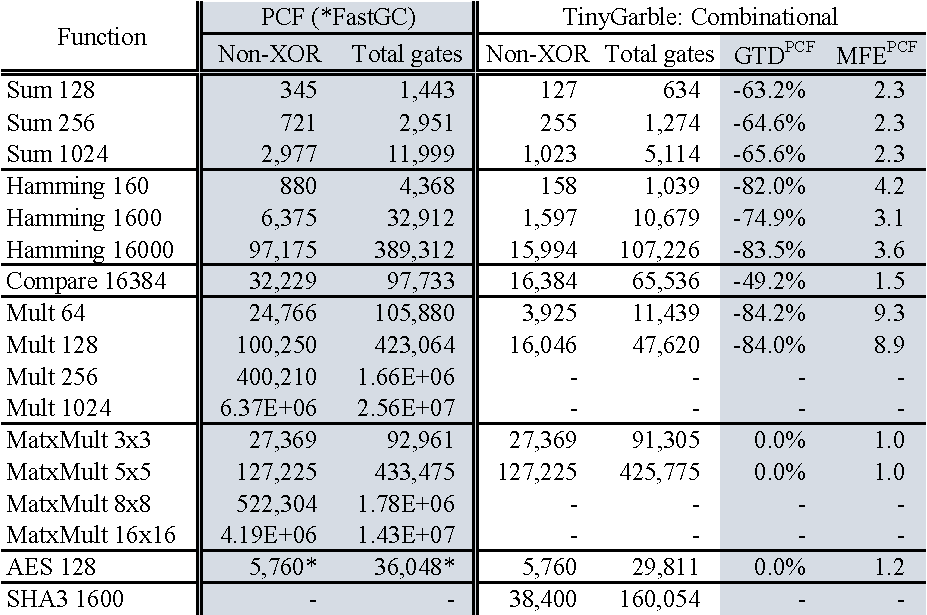
\includegraphics[width=0.7\textwidth]{results-comb-crop.pdf}
\end{table*}

\begin{table*}
\centering
\caption{Comparison of TinyGarble sequential circuits with PCF and TinyGarble combinational circuits.
In case of AES 128, the result is compared with FastGC.}
\label{table:result-seq}
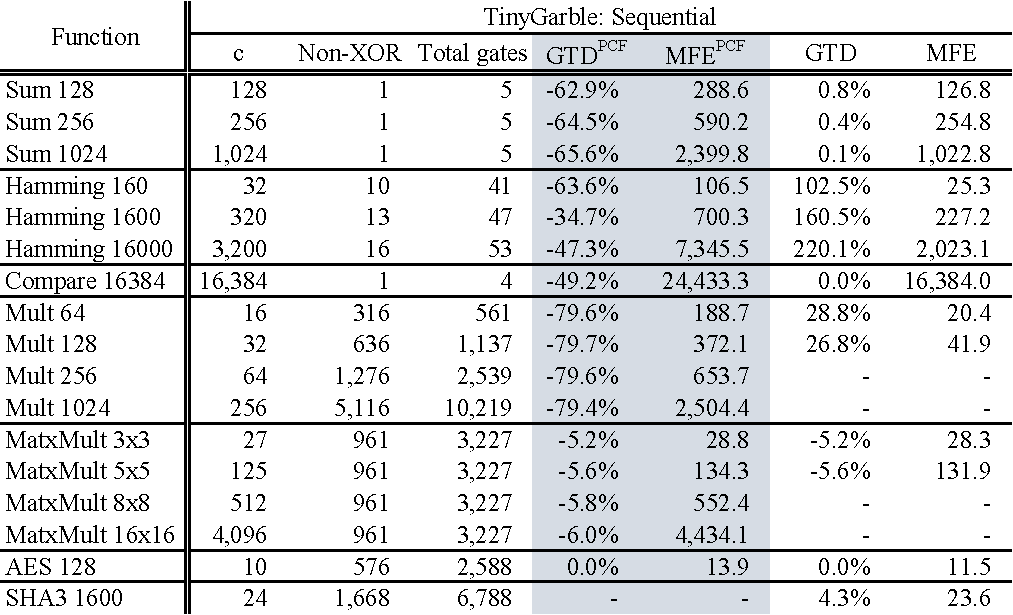
\includegraphics[width=0.7\textwidth]{results-seq-crop.pdf}
\end{table*}

\tab{table:result-seq} shows the number of total gates, non-XOR gates, $\mathit{MFE}$, $\mathit{GTD}$, $\mathit{MFE}$\textsuperscript{PCF}, and $\mathit{GTD}$\textsuperscript{PCF} of the benchmark circuits for various input widths.
$\mathit{MFE}$, $\mathit{GTD}$ are computed with TinyGarble combinational circuits (with $c=1$) as reference.
$\mathit{MFE}$\textsuperscript{PCF}, and $\mathit{GTD}$\textsuperscript{PCF} use the circuits reported in PCF as reference.
In the case of AES 128, we compare our implementation with the manually optimized circuit reported in FastGC \cite{huang2011faster} because PCF did not report it directly.

We provide a few highlights from \tab{table:result-seq}.
TinyGarble is able to decrease the size of the sum of two $1024$-bit numbers by $\numprint{1022.8}$ times (i.e., more than three orders of magnitude) without affecting the number of garbled tables ($\mathit{GTD}$) compared with its own combinational circuit.
For Hamming 16000, TinyGarble is able to decrease the memory footprint by $\numprint{7345.5}$ times (i.e., about 4 orders of magnitude) while reducing the number of garbled tables by $47.3\%$ in comparison with the circuit reported in PCF.
In case of Mult 1024, TinyGarble shrinks the memory footprint by a factor of $\numprint{2504.4}$ while reducing the number of garbled tables by $79.4\%$ when compared with the result in PCF.
For a $16\times 16$ matrix multiplication, a $\numprint{4434.1}$ more compact TinyGarble solution with $6\%$ less garbled tables compared with PCF is available.
By folding AES-128 10 times, the total number of gates is reduce by a factor of $13.9$ compared to the  FastGC circuit without any overhead in the number of non-XORs.
Observe that the savings are typically more for larger bit-widths while extreme foldings can introduce an increased overhead in number of garbled tables due to the resulting asymmetry.

Because of the TinyGarble superior scalability, we are able to implement functions that have never been reported before, such as SHA-3, which can be represented using $\numprint{344059}$ and $\numprint{6788}$ gates respectively.

\section{Effect of Folding on Garbling Time}
So far, we have only reported the overhead in terms of garbled tables ($\mathit{GTD}$) that is a function of the number of non-XOR gates.
As explained in \cite{bellare2013efficient}, if we see garbling as a cryptographic primitive, its computation time (without considering communication) will also be interesting.
In practice, smaller circuits which can fit entirely in the processor cache result in fewer cache misses and therefore, consume less CPU cycles for garbling.
To better observe the impact of cache speed-up for the compact circuits resulting from TinyGarble, \fig{fig:cpu_time} depicts the CPU Time (left y-axis) and the memory footprint of wire tokens (right y-axis) versus $c$ (x-axis) for the $\numprint{32768}$-bit Sum function.
As mentioned earlier, the memory footprint is directly proportional to the total number of gates in the sequential circuit.

This experiment is done using our sequential garbling scheme based on JustGarble \cite{bellare2013efficient} that includes using Free XOR, Row Reduction, and Fixed-key AES garbling techniques (see \sect{subsect:preli_GC}).
We use an Intel Core i7 CPU @ 3.40GHz which supports the AES-NI instruction set.
The CPU cycle is measured as the average of $10,000$ trials using RDTSC instruction.
For security parameter $k=128$ (the bit-width of wire token, see \sect{subsect:preli_GC}), we store $128$-bit per tokens.
For garbling in JustGarble, we store 2 tokens, 2 32-bit input indexes, and an 8-bit gate-type per gate.
Thus, the memory footprint is approximately $328$-bit per gate in garbling operation.
Folding the circuit by a factor of $c \in [1:\numprint{32768}]$ constantly decreases the memory footprint while the computation effort remains almost constant.
Interestingly, as can be seen from the figure, the number of CPU cycles sharply decreases by $1.6\times$ just when we fold four times ($c=4$) compared to $c=1$.
This is because for $c \geq 4$, the memory space required for garbling completely fits in the cache.
The minimum CPU cycle per gate happens at $c=\numprint{2048}$ for $3.2$~KB memory footprint.
This signifies the fact that even for large functions, we can use the sequential approach to fit the corresponding memory space requirement into the cache and avoid the penalty of cache misses, thus achieving a large reduction in garbling time.

\begin{figure}[ht]
	\centering
	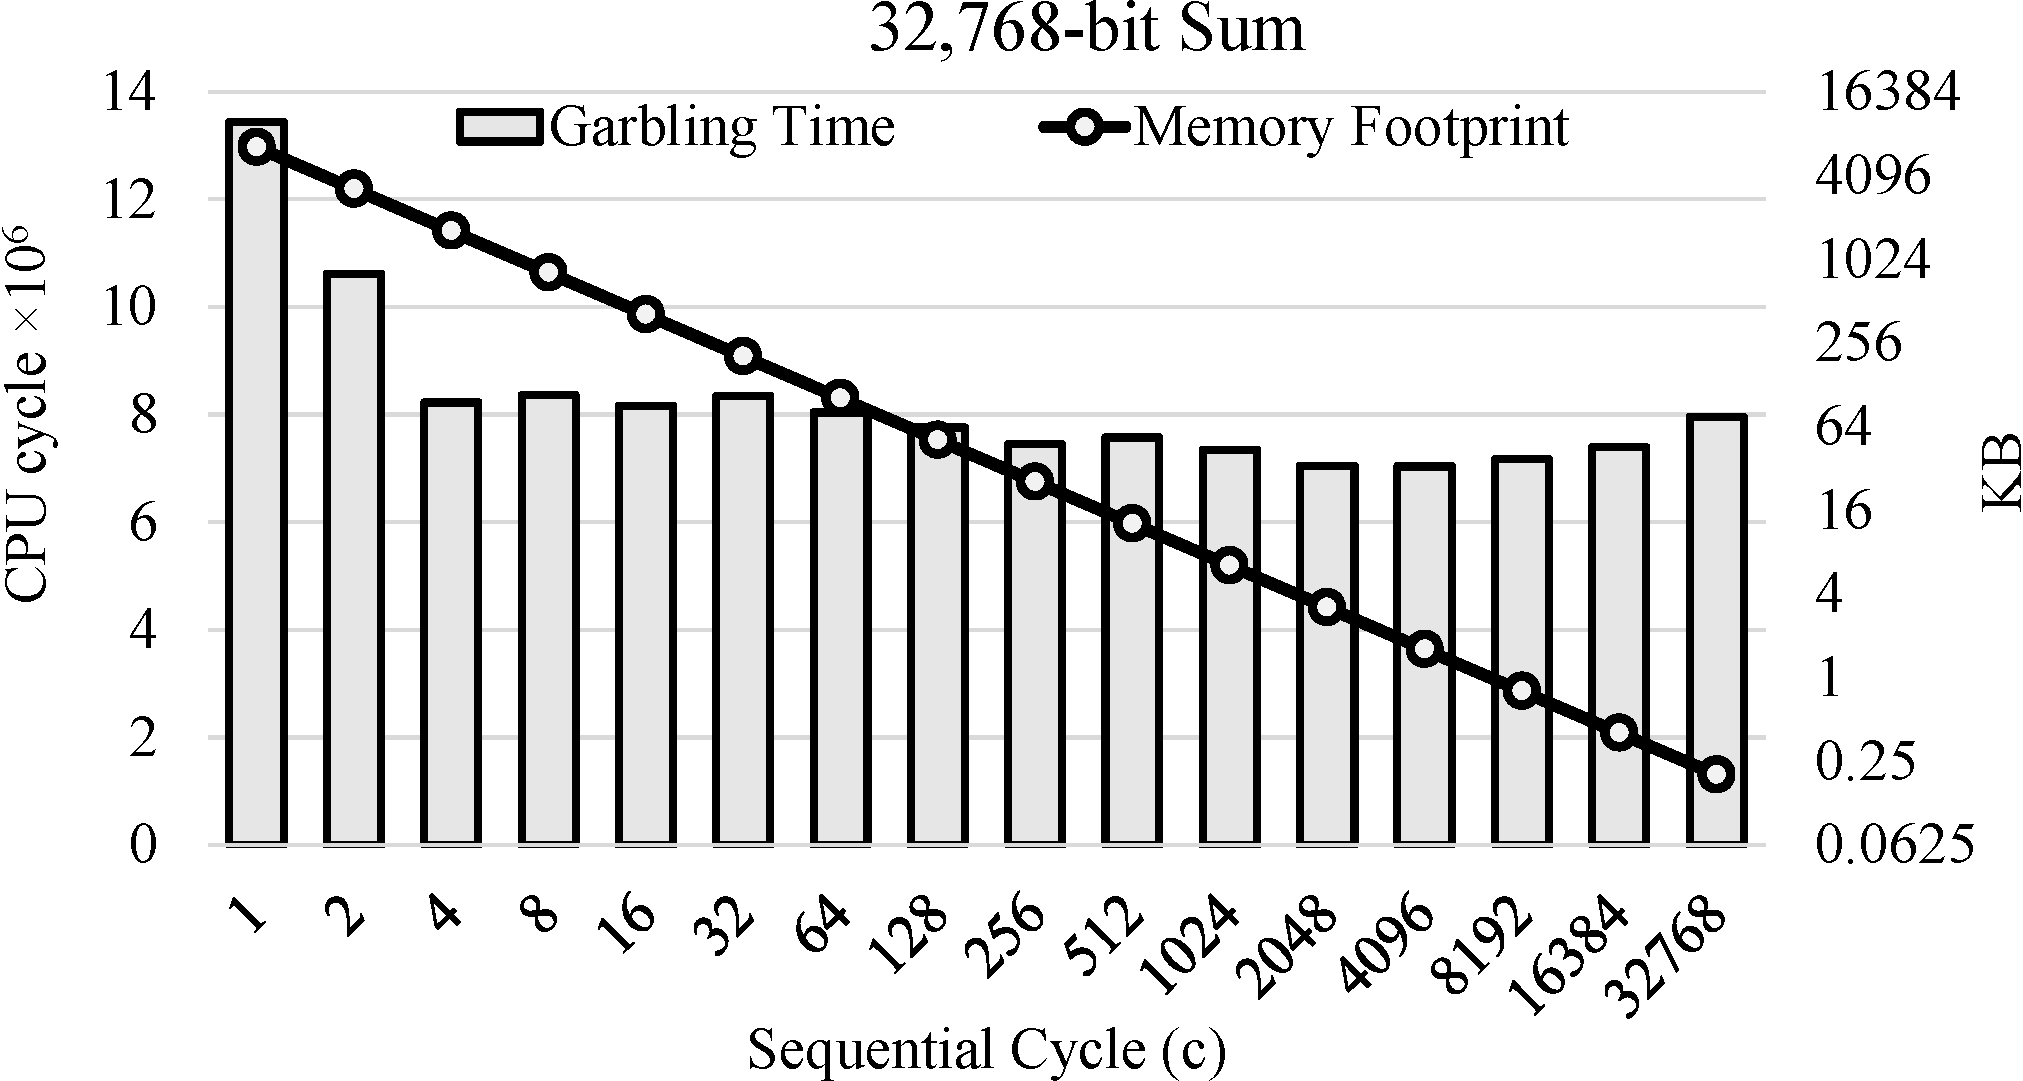
\includegraphics[width=0.7\textwidth]{CPU_Time-crop.pdf}
	\caption{Garbling $\numprint{32768}$-bit Sum function.
The CPU time in number of cycles and the approximate memory footprint in KBytes (y-axis) versus $c$ (x-axis) are shown.}
	\label{fig:cpu_time}
\end{figure}

\section{High Level Synthesis Tools}
The design automation community has been working on tools that work with higher-level languages and abstractions than HDL.
While a host of commercial and academic HLS tools are available \cite{tool:Vivado, tool:PandA, decaluwe2004myhdl, Gupta2004}, we selected the Xilinx Vivado HLS for compiling C code to HDL which can then be synthesized using a conventional HDL synthesis tool.
The HLS engine in the Vivado suite is built upon the xPilot project \cite{Chapter:Zhang2008}.

\begin{table*}[t]
\centering
\caption{Comparison of performance of the circuits generated using C input to HLS and a direct Verilog input to the HDL synthesizer.}
\label{table:hls}
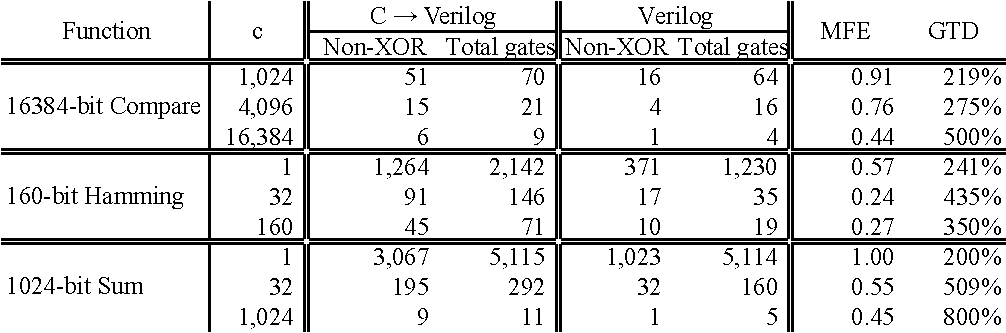
\includegraphics[width=0.7\textwidth]{HLS-crop.pdf}
\end{table*}

Table \ref{table:hls} demonstrates a comparison between the performance of the circuits generated using C input to the HLS tool (C$\rightarrow$Verilog) and a direct Verilog input.
As can be seen from the table, the resulting memory footprint could increase by a factor between 1 and 4, while the number of garbled tables varies in a range of 3 to 9 times.
It is well known that writing the HDL level code which contains the time information and more detailed structural/behavioral description would yield much more efficient circuits than the code written in a higher level language.

\section{Evaluation of MIPS}
We implement general purpose processor for \acrshort{pf-sfe} using MIPS~I where one user provide function description in assembly and the other provides the data.
Support of sequential circuits in TinyGarble enables us to use the MIPS circuit description in Plasma project \cite{rhoads2006plasma} without major modifications.
In the following, we provide the result of MIPS implementation and its memory footprint and communication load.
Lastly, we present implementation of Hamming distance with variable input length as a benchmark of private function application on MIPS.

\subsection{MIPS Implementation}
We used TinyGarble to generate the netlist for the MIPS sequential circuit.
\tab{table:mipsres} shows the total number of gates and non-XOR gates for each module of the MIPS processor with $64\times32$bit DM and IM.
The sum of non-XORs for each module is $\numprint{14997}$.
However, when the modules are combined together to form the entire MIPS processor, the synthesizer optimizes the circuit such that the total number of non-XORs is reduced by $14.95\%$ to $\numprint{12755}$.
The memory footprint for storing tokens during garbling MIPS is approximately the size of two tokens times the total number of gates which is $2 \times 128 \times \numprint{31719}$bit $=991$~KB for token bit-width $k=128$.
The communication load between parties for invocation of one instruction (one sequential cycle) is approximately the size of three tokens times the number of non-XOR gates which is $3\times 128 \times \numprint{12755}$bit $=598$~KB with Row Reduction optimization.

\begin{table}[ht]
\centering
\caption{Number of total gates and non-XOR gates in the MIPS implementation.
The global optimization of TinyGarble reduces the overall number of gates compared to that of the sum of individual modules.}\label{table:mipsres}
\begin{tabular}{l|rrl}
Modules             & Total gates & Non-XOR \\ \hline \hline
Controller          & 509                                                  & 470                                                \\
Bus                 & 603                                                  & 590                                                \\
ALU                 & 651                                                  & 346                                                \\
Shifter             & \numprint{1362}                                                 & \numprint{1092}                                               \\
Mult                & \numprint{2147}                                                 & \numprint{1792}                                               \\
Reg File            & \numprint{8880}                                                 & \numprint{3023}                                               \\
IM                  & \numprint{6048}                                                 & \numprint{2016}                                               \\
DM                  & \numprint{13779}                                                & \numprint{5423}                                               \\
PC                  & 309                                                  & 245                                                \\ \hline
Total               & \numprint{34288}                                                & \numprint{14997}                                              \\ \hline \hline
MIPS                & \numprint{31719}                                                & \numprint{12755}                                              \\ \hline \hline
\begin{tabular}[c]{@{}l@{}}Global \\optimization\end{tabular} & 7.49\%                                               & 14.95\%
\end{tabular}
\end{table}

\subsection{Benchmark: Hamming Distance}
We implemented the Hamming distance function as a proof-of-concept for our secure MIPS.
It counts the number of different elements in two arrays $A$ and $B$ with variable length $l$.
For the hand-optimized assembly code shown in \fig{figure:hamminassembly}, the function requires at most $7+9l$ sequential cycles (instructions) to evaluate.
Thus, based on \tab{table:mipsres}, this function requires overall $\numprint{12755}\times(7+9l)$ non-XOR gates.
It has only $16$ instructions and is stored in $16\times32$bit of the IM.
The function requires that $l$, $A$, and $B$ are stored in addresses $0$, $[2:l+1]$, and $[l+2:2l+1]$ of DM respectively.
It will store the Hamming distance of $A$ and $B$ in address $1$.

\begin{figure}[ht]
\lstinputlisting{Hamming.s}
\caption{Hamming distance assembly code.}\label{figure:hamminassembly}
\end{figure}

\section{Open Source Logic Synthesis Tools}
TinyGarble offers a generic methodology for generating GC that is transparent to the underlying logic synthesis tool.
To show this point, we demonstrate an implementation of TinyGarble using the Yosys \cite{tool:Yosys} and ABC \cite{tool:ABC} logic synthesis tool chain for circuit generation.
Both of these tools are open-source and available online.
We compare the performance of the commercial HDL synthesis tool, i.e., Synopsys DC, with this open-source synthesis tool chain.
ABC is an academic package developed at the University of California Berkeley.
Yosys is an HDL-based synthesis tool which calls ABC for its technology mapping.
The HDL inputs for describing both sequential and combinational circuits are written in the Verilog programming language.

We compare the performance of these open-source tools to the commercially available Synopsys DC.
The results are presented in \tab{table:abc}.
For comparison purposes, we compute $\mathit{GTD}$ and $\mathit{MFE}$ using the netlists generated by Synopsys DC as reference.
For most of the benchmarks $\mathit{GTD}$s are either very small or zero which implies that the number of non-XOR gates in circuits generated by Yosys and by Synopsys DC are almost similar.
In terms of memory footprint, different tools perform better for different benchmark functions.
These results shows that TinyGarble is transparent to the underlying logic synthesis tool as long as the tool is up to date with respect to the known methods for logic minimization and mapping.
Since the logic synthesis tools perform a series of optimizations, they may use different (heuristic) algorithms for some of their internal steps which could lead to slightly different results.
A user can choose between different synthesis tools based on their performance and availability.

\begin{table}[ht]
\caption{Comparison of circuit generation performance between the commercial Synopsys DC and Yosys+ABC open source logic synthesizer.}
\label{table:abc}
\centering
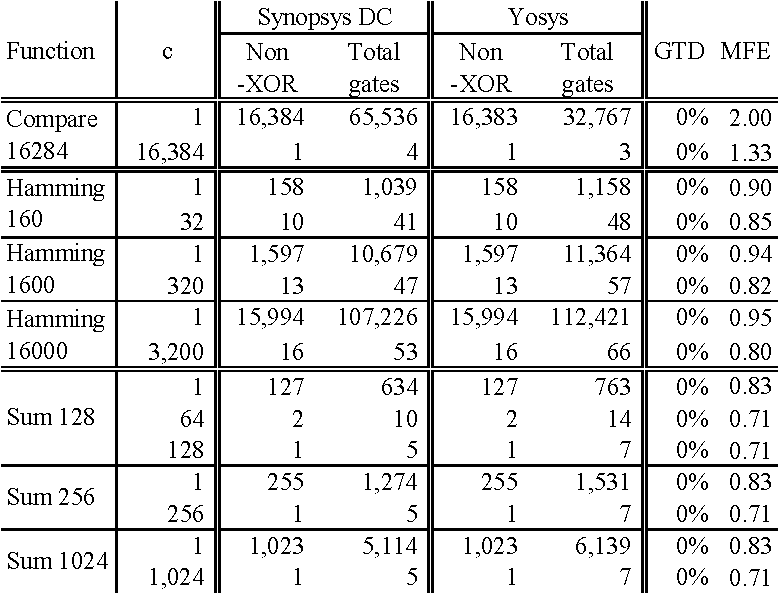
\includegraphics[width=0.7\textwidth]{abc-crop.pdf}
\end{table}

\section{Evaluation Setup of GarbledCPU}\label{ssect:evalset}
We create different instances of a single-cycle MIPS architecture with specific, restricted, and full IS to support a trade-off between efficiency and privacy. (Full IS was proposed in \cite{songhori2015tinygarble} and is reported for comparison.) The different MIPS instances are synthesized using Synopsys Design Compiler DC H-2013.03-SP4 to generate optimized sequential Boolean circuits. These circuits are then evaluated on our hardware GC evaluator implemented using Vivado 2014.4.1 on a Xilinx Virtex-7 FPGA.

\section{Benchmarks}\label{ssect:bench}
As benchmarks we used Hamming distance, private set intersection and AES. We compile these benchmarks from high-level C to MIPS binary using a MIPS cross-compiler. For some benchmarks, assembly code manipulation allows to reduce the number of clock cycles required. To assure correctness of both benchmarks and IS under test, we simulate the resulting binary file using the Modelsim simulator and calculate the number of required cycles to compute each of the benchmarks, reported in~\tab{tab:cyc_bench}, for accurate performance measurements. For Hamming distance, the number of cycles depends on the size of the input strings. In the PSI benchmark, we compute a variant of PSI called PSI cardinality (PSI-CA) where only the number of common elements is revealed. The sets can have different sizes where each element is 32-bit.  For AES, we assume that one party holds a 128-bit message and the other party holds eleven round keys each of 128-bit length to avoid unnecessary garbling and evaluation of the round-key generation function.

\begin{table}[ht]
\caption{Number of required cycles to compute benchmarks.}\label{tab:cyc_bench}
\centering
\small
\begin{tabular}{l|r|r}
\multicolumn{1}{c|}{Benchmark} & \multicolumn{1}{c|}{Input Size} &  \multicolumn{1}{c}{\# of required cycles} \\
\hline
\hline
Hamming Distance & $\numprint{16}$ & $\numprint{218}$\\
\hline
 Hamming Distance & $\numprint{32}$ & $\numprint{426}$\\
\hline
Hamming Distance & $\numprint{64}$ & $\numprint{842}$\\
\hline
Hamming Distance & $\numprint{128}$ & $\numprint{1674}$\\
\hline
PSI & $\numprint{64}$ &$\numprint{7267}$\\
\hline
PSI & $\numprint{128}$ &$\numprint{14267}$\\
\hline
AES (no key expansion) & $\numprint{128}$ & $\numprint{6178}$\\
\end{tabular}
\end{table}

\section{Synthesis of the GarbledCPU IS}
We synthesize the MIPS architecture, shown in~\fig{figure:mips}, with Synopsys DC for different ISs and memory sizes: 32 to 512 32-bit words for instruction and data memories. Generating these Boolean circuits is a one-time process and the circuits can be re-used without incurring further compilation costs. \tab{tab:synres} shows the synthesis time and number of non-XOR gates of the IS's with different sizes of memories.

\begin{table}[ht]
\caption{Synthesis results of different variants of (IS)}\label{tab:synres}
\centering
\begin{tabular}{l|r|r|r}
\multicolumn{1}{c|}{Memory Size} & \multicolumn{1}{c|}{Synthesis Time} &  \multicolumn{1}{c|}{\# of Combinatorial} & \multicolumn{1}{c}{\# of Sequential} \\
\multicolumn{1}{c|}{(words)} & \multicolumn{1}{c|}{seconds (s)} &  \multicolumn{1}{c|}{non-XOR gates} & \multicolumn{1}{c}{gates} \\
\hline
\hline
\multicolumn{4} {c}{Hamming Distance-specific IS}\\
\hline
DM, IM = 32 & $\numprint{19.648}$~$s$ & $\numprint{6715}$ & $\numprint{2021}$ \\
\hline
DM, IM = 64 & $\numprint{31.692}$~$s$ & $\numprint{9830}$ & $\numprint{3046}$ \\
\hline
DM, IM = 128 & $\numprint{62.212}$~$s$ & $\numprint{16062}$ & $\numprint{5095}$ \\
\hline
DM, IM = 256 & $\numprint{167.398}$~$s$ & $\numprint{28493}$ & $\numprint{9192}$ \\
\hline
DM, IM = 512 & $\numprint{589.186}$~$s$ & $\numprint{53374}$ & $\numprint{17385}$ \\
\hline
\multicolumn{4} {c}{PSI-specific IS}\\
\hline
DM, IM = 32 & $\numprint{18.735}$~$s$ & $\numprint{6751}$ & $\numprint{2021}$ \\
\hline
DM, IM = 64 & $\numprint{31.117}$~$s$ & $\numprint{9866}$ & $\numprint{3046}$ \\
\hline
DM, IM = 128 & $\numprint{61.551}$~$s$ & $\numprint{16097}$ & $\numprint{5095}$ \\
\hline
DM, IM = 256 & $\numprint{163.564}$~$s$ &$\numprint{28529}$ & $\numprint{9192}$ \\
\hline
DM, IM = 512 & $\numprint{591.145}$~$s$ & $\numprint{53410}$ & $\numprint{17385}$ \\
\hline
\multicolumn{4} {c}{AES-specific IS}\\
\hline
DM, IM = 256 & $\numprint{169.498}$~$s$ &$\numprint{32177}$ & $\numprint{9214}$ \\
\hline
DM, IM = 512 & $\numprint{594.047}$~$s$ & $\numprint{61570}$ & $\numprint{17406}$\\
\hline
\multicolumn{4} {c}{ALU\&Shift IS}\\
\hline
DM, IM = 32 & $\numprint{21.681}$~$s$ & $\numprint{9676}$ & $\numprint{2046}$ \\
\hline
DM, IM = 64 & $\numprint{34.588}$~$s$ & $\numprint{12702}$ & $\numprint{3070}$ \\
\hline
DM, IM = 128 & $\numprint{65.873}$~$s$ & $\numprint{19694}$ & $\numprint{5118}$ \\
\hline
DM, IM = 256 & $\numprint{170.974}$~$s$ &$\numprint{34071}$ & $\numprint{9214}$ \\
\hline
DM, IM = 512 & $\numprint{593.945}$~$s$ & $\numprint{66238}$ & $\numprint{17406}$ \\
\hline
\multicolumn{4} {c}{ALU-only IS}\\
\hline
DM, IM = 32 & $\numprint{19.599}$~$s$ & $\numprint{8136}$ & $\numprint{2046}$ \\
\hline
DM, IM = 64 & $\numprint{31.970}$~$s$ & $\numprint{11696}$ & $\numprint{3070}$ \\
\hline
DM, IM = 128 & $\numprint{62.599}$~$s$ & $\numprint{18816}$ & $\numprint{5118}$ \\
\hline
DM, IM = 256 & $\numprint{164.894}$~$s$ &$\numprint{33041}$ & $\numprint{9214}$ \\
\hline
DM, IM = 512 & $\numprint{598.986}$~$s$ & $\numprint{65183}$ & $\numprint{17406}$ \\
\hline
\multicolumn{4} {c}{Full IS~\cite{songhori2015tinygarble}}\\
\hline
DM, IM = 32 & $\numprint{38.331}$~$s$ & $\numprint{13257}$ & $\numprint{2110}$ \\
\hline
DM, IM = 64 & $\numprint{50.446}$~$s$ & $\numprint{16818}$ & $\numprint{3134}$ \\
\hline
DM, IM = 128 & $\numprint{82.863}$~$s$ & $\numprint{23899}$ & $\numprint{5182}$ \\
\hline
DM, IM = 256 & $\numprint{189.157}$~$s$ &$\numprint{38118}$ & $\numprint{9278}$ \\
\hline
DM, IM = 512 & $\numprint{616.750}$~$s$ & $\numprint{69423}$ & $\numprint{17470}$ \\
\end{tabular}
\end{table}


\begin{itemize}
\item \emph{Application-specific IS for public functions:} We synthesized three variants of the application-specific IS where the selected instructions include only the ones used by a particular function, for various memory sizes. We create the application-specific IS for the three benchmarks: Hamming distance\footnote{\small{Instructions required for \emph{Hamming distance} are:} \tiny{LW, SW, ADD, SUB, XOR, NOP, SLL and BEQ}}, PSI\footnote{\small{Instructions required for \emph{PSI} are:} \tiny{LW, SW, ADD, SUB, NOP, SLL, BEQ, BNE and SLT}}, and AES\footnote{ \small{Instructions required for \emph{AES} are:} \tiny{LW, LB, SW, SB, ADD, SUB, AND, XOR, OR, NOP, SLL, SRL, BEQ, BNE, JAL, JR and SLT}}.
\item \emph{Restricted IS for semi-private functions:} We synthesized two variants of the restricted IS: one without the Mult/Div unit and another without Mult/Div and Shift units. Since the difference between the two depends mainly on reducing the control logic and select lines of multiplexers, the numbers of non-XOR gates for both are different. However, the number of flip-flops are the same.
\item \emph{Full IS~\cite{songhori2015tinygarble} for private functions:} We show full IS synthesis results with different memory sizes in \tab{tab:synres}.
\end{itemize}

\section{Performance Evaluation}
\subsection{Area} \tab{table:resource} shows the resource allocation and utilization of our GC Evaluator on a Xilinx Virtex-7 FPGA. Note that the FPGA utilization does not vary for different memory sizes and instances of the MIPS processor since the evaluator logic remains unaltered. For different memory sizes and IS instances, only the non-XOR gate count varies. This only impacts the garbled labels and tables memory which significantly affects the off-chip memory utilized for storing the garbled tables, and the Block Random-Access Memory (BRAM) resources utilization only to a small extent.

\begin{table}[ht]
\centering
\caption{Resource allocation and utilization of GarbledCPU GC Evaluator on a Xilinx Virtex-7 FPGA.}
\label{table:resource}
\begin{tabular}{l|r|r}
Resource    & \multicolumn{1}{c|}{Estimation} & \multicolumn{1}{c}{Utilization \%} \\ \hline \hline
Flip-Flop (FF) & $\numprint{22035}$ & $\numprint{2.54}$ \\ \hline
Slice LookUp Table (LUT) & $\numprint{21229}$ & $\numprint{4.90}$ \\ \hline
BRAM & $\numprint{354}$ & $\numprint{24}$
\\ \hline
BUFG & $\numprint{2}$ & $\numprint{6.25}$
 \end{tabular}
\end{table}

\subsection{Performance} \tab{table:performance} presents the runtime required to evaluate GarbledCPU for one instruction in terms of clock cycles and $\mu\textrm{s}$. Our GC evaluator operates at $100\textrm{MHz}$ on the FPGA. This is used to compute an average evaluation runtime of 1.1 clock cycles per gate for our pipelined GC evaluator which translates to an average of $11\textrm{ns}$ per gate in our FPGA implementation. The reported runtime can be further improved by providing tighter timing constraints.

\subsection{Comparison with Other Work}
\tab{tab:comp} shows a comparison with other GC evaluator implementations. However, for fairness, we are leveraging GC optimizations that were not available at the time for \cite{jarvinen2010garbled}. We compare with our two implementations, the 21-stage pipelined evaluator and un-pipelined variant to show the effect of pipelining in improving our performance by a factor of 7.8. \tab{tab:comp} compares our results with interpolated results estimated for other works. Results indicate that our pipelined GC evaluator FPGA implementation takes $51\times$ fewer clock cycles compared to the fastest software implementation JustGarble \cite{bellare2013efficient}. Although the CPU clock frequency ($3.0\textrm{GHz}$) is $30\times$ faster than that of our Virtex-7 FPGA ($100\textrm{MHz}$), our pipelined implementation would still be almost $2\times$ faster than JustGarble in terms of absolute time. Note that our implementation is just a prototype on a reconfigurable FPGA as opposed to a custom design of Intel AES-NI in CPU. Implementing GarbledCPU on an ASIC would improve its performance in terms of absolute time even further. Moreover, our implementation is two orders of magnitude faster than the previously fastest hardware implementation of \cite{jarvinen2010garbled}.

\begin{table}[ht]
\centering
\caption{Performance of GarbledCPU for different (ISs) with different memory sizes at $100\textrm{MHz}$ clock frequency.}\label{table:performance}
\begin{tabular}{l|r|r|r|r|r}
\multicolumn{1}{c|}{Memory Size (words)} & \multicolumn{1}{c|}{$\numprint{32}$ } &  \multicolumn{1}{c|}{$\numprint{64}$ } & \multicolumn{1}{c|}{$\numprint{128}$ } & \multicolumn{1}{c|}{$\numprint{256}$ } & \multicolumn{1}{c}{$\numprint{512}$ }  \\ \hline \hline
\multicolumn{6} {c}{Hamming Distance-IS}\\ \hline
\# of non-XOR gates       & $\numprint{6715}$    & $\numprint{9830}$   & $\numprint{16062}$ & $\numprint{28493}$ & $\numprint{53374}$\\ \hline
Time per inst. (cc)       & $\numprint{7118}$    & $\numprint{10813}$ & $\numprint{17829}$ & $\numprint{30773}$  & $\numprint{57644}$\\ \hline
Time per inst. ($\mu s$) & $\numprint{71.18}$  & $\numprint{108.13}$  & $\numprint{178.29}$  & $\numprint{307.72}$  & $\numprint{576.44}$\\ \hline
Avg. Time per gate (cc)  & $\numprint{1.06}$      & $\numprint{1.10}$   & $\numprint{1.11}$    & $\numprint{1.08}$  & $\numprint{1.08}$\\ \hline
\multicolumn{6} {c}{PSI-IS}\\ \hline
\# of non-XOR gates       & $\numprint{6751}$    & $\numprint{9866}$   & $\numprint{16097}$ & $\numprint{28529}$ & $\numprint{53410}$\\ \hline
Time per inst. (cc)       & $\numprint{7426}$    & $\numprint{10952}$ & $\numprint{18029}$ & $\numprint{30811}$  & $\numprint{57149}$\\ \hline
Time per inst. ($\mu s$) & $\numprint{74.26}$  & $\numprint{109.52}$  & $\numprint{180.29}$  & $\numprint{308.11}$  & $\numprint{571.49}$\\ \hline
Avg. Time per gate (cc)  & $\numprint{1.10}$      & $\numprint{1.11}$   & $\numprint{1.12}$    & $\numprint{1.08}$  & $\numprint{1.07}$\\ \hline
\multicolumn{6} {c}{AES-specific IS}\\ \hline
\# of non-XOR gates       & - & -&- & $\numprint{32177}$   & $\numprint{61570}$\\ \hline
Time per inst. (cc)       &-  & -&- & $\numprint{35717}$   & $\numprint{68343}$\\ \hline
Time per inst. ($\mu s$) & - & -& -& $\numprint{357.17}$ & $\numprint{683.43}$ \\ \hline
Avg. Time per gate (cc)  & -&- &- & $\numprint{1.11}$      & $\numprint{1.11}$ \\ \hline
\multicolumn{6} {c}{ALU\&Shift-IS}\\
\hline
\# of non-XOR gates       & $\numprint{9676}$    & $\numprint{12702}$ & $\numprint{19694}$ & $\numprint{34071}$  & $\numprint{66238}$\\ \hline
Time per inst. (cc)       & $\numprint{10644}$  & $\numprint{13972}$ & $\numprint{22057}$ & $\numprint{36115}$  & $\numprint{71537}$\\ \hline
Time per inst. ($\mu s$) & $\numprint{106.44}$ & $\numprint{139.72}$  & $\numprint{220.57}$  & $\numprint{361.15}$  & $\numprint{715.37}$\\ \hline
Avg. Time per gate (cc)  & $\numprint{1.10}$     & $\numprint{1.10}$   & $\numprint{1.12}$    & $\numprint{1.06}$  & $\numprint{1.08}$\\ \hline
\multicolumn{6} {c}{ALU-only IS}\\
\hline
\# of non-XOR gates       & $\numprint{8136}$    & $\numprint{11696}$   & $\numprint{18816}$  & $\numprint{33041}$ & $\numprint{65183}$\\ \hline
Time per inst. (cc)       & $\numprint{8624}$  & $\numprint{12866}$ & $\numprint{21074}$  & $\numprint{35684}$  & $\numprint{73657}$\\ \hline
Time per inst. ($\mu s$) & $\numprint{86.24}$ & $\numprint{128.66}$     & $\numprint{210.74}$  & $\numprint{356.84}$  & $\numprint{736.57}$\\ \hline
Avg. Time per gate (cc)  & $\numprint{1.06}$     & $\numprint{1.10}$    & $\numprint{1.12}$    & $\numprint{1.08}$  & $\numprint{1.13}$\\ \hline
\multicolumn{6} {c}{Full IS~\cite{songhori2015tinygarble}}\\
\hline
\# of non-XOR gates       & $\numprint{13257}$    & $\numprint{16818}$   & $\numprint{23899}$ & $\numprint{38118}$ & $\numprint{69423}$\\ \hline
Time per inst. (cc)       & $\numprint{14848}$  & $\numprint{18668}$ & $\numprint{25811}$ & $\numprint{40786}$  & $\numprint{77060}$\\ \hline
Time per inst. ($\mu s$) & $\numprint{148.48}$ & $\numprint{186.68}$  & $\numprint{258.11}$  & $\numprint{407.86}$  & $\numprint{770.60}$\\ \hline
Avg. Time per gate (cc)  & $\numprint{1.12}$     & $\numprint{1.11}$   & $\numprint{1.08}$    & $\numprint{1.07}$  & $\numprint{1.11}$\\
\end{tabular}
\end{table}

\begin{table}[ht]
\centering
\caption{Comparing our GC evaluator implementation with other works' estimation for MIPS with 64-word memory.}\label{tab:comp}
\begin{tabular}{l||r|r}
\multicolumn{1}{c||}{Method} & \multicolumn{1}{c|}{\begin{tabular}[c]{@{}c@{}}Total time\\(cc)\end{tabular}} & \multicolumn{1}{c}{cc/gate} \\ \hline \hline
J\"arvinen et al. (SoC)~\cite{jarvinen2010garbled} & $\numprint{37329233}$ & $\numprint{2219.6}$ \\ \hline
J\"arvinen et al. (Stand-Alone FPGA)~\cite{jarvinen2010garbled} & $\numprint{4291954}$ & $\numprint{255.2}$ \\ \hline
JustGarble (CPU)~\cite{bellare2013efficient} & $\numprint{948535}$ & $\numprint{56.4}$ \\ \hline
Our work w/o pipeline & $\numprint{144635}$ & $\numprint{8.6}$ \\ \hline
Our work w/ pipeline & $\numprint{18500}$ & $\numprint{1.1}$
\end{tabular}
\end{table}

\section{Evaluation of ARM2GC}\label{sec:eval}
We also compare the overall performance of our GarbledCPU with the performance of the proposed software solution in \cite{wang2016secure} on the compatible benchmarks. For computing Hamming distance on two 32-bit integer arrays, Wang et al.'s solution takes $1.24s$ to garble 481K gates (see Table 4 in \cite{wang2016secure}). GarbledCPU requires \numprint{6715} non-XOR gates and \numprint{426} cycles (see Tables \ref{tab:synres} and \ref{tab:cyc_bench}), and thus it takes only $0.0314s$ to evaluate 2.8M gates. Given that garbling time is double the evaluation time, this indicates a speedup of factor 18 for GarbledCPU but with $6\times$ more AND gates for the same functionality. In terms of throughput, GarbledCPU can evaluate 90.8M gates and Wang et al.'s solution can evaluate 776K gates which makes GarbledCPU 117 times faster owing to our hardware implementation. However, this speedup assumes on-chip memory and is likely to be much smaller when utilizing off-chip memory.

\subsection{Evaluation Setup}
We use Synopsis Design Compiler (DC) H-2013.03-SP4~\cite{tool:DesignCompiler} along with TinyGarble~\cite{songhori2015tinygarble} synthesis and technology libraries to generate the netlists for the benchmark circuits and the ARM processor.

For the ARM2GC framework, we use the Amber ARM project, an open-source implementation of ARM v2a ISA on opencores~\cite{santifort2010amber}.
The ARM circuit is modified as explained in \sect{ssec:arm}.
Synthesizing the ARM processor with Synopsis DC takes few hours.
However, the process is done only once for a given memory size and it can be used for any set of functions and inputs afterwards.
The benchmark functions for ARM2GC are implemented in C and compiled using GNU gcc-arm-linux-gnueabi (Ubuntu/Linaro 5.3.1-14ubuntu2).
We used \texttt{-Os} compiler optimization flag in order to reduce the number of instructions.
We modified the header assembly code to change the addresses of stack, code, and data memories in the compiled binary.
We do not apply any optimization on the binary code.
Thus, similar to a normal software compilation, it takes less than a few seconds to compile a function into an ARM binary code.

\subsection{Benchmark Functions and Metrics}
We use the benchmark functions that have been frequently used for evaluation in the GC literature~\cite{holzer2012secure, songhori2015tinygarble, wang2016secure}. The benchmarks are as follows:

\begin{itemize}
\vspace{-0.06in}
\item Sum adds two integers.
\vspace{-0.1in}
\item Compare compares two integers.
\vspace{-0.1in}
\item Hamming finds the Hamming distance between two integers.
\vspace{-0.1in}
\item Mult calculates the product of two integers.
\vspace{-0.1in}
\item MatrixMult$N\times N$ computes matrix multiplication of two $N\times N$ matrices.
\vspace{-0.1in}
\item SHA3 finds SHA3-256 hash of a string.
\vspace{-0.1in}
\item AES computes AES-128 encryption given two 128-bit numbers as the key and the message.
\end{itemize}

%Metric
The most important metric to compare the cost of garbling is the total number of garbled non-XOR gates.
This metric encompasses both the cost of computation (encrypting/decrypting garbled tables) and the cost of communication (transferring garbled tables) in the GC protocol \cite{kolesnikov2008improved}.

\begin{table}
\centering
\caption{SkipGate algorithm improvement on sequential circuits generated by TinyGarble (TG)~\cite{songhori2015tinygarble}. These functions do not have public inputs. SkipGate benefits from the small number of flip-flops initial values that are public to reduce their garbling cost.}\label{tab:sys_impvoment}
\resizebox{\columnwidth}{!}{%
\begin{tabular}{l||r|r|r||r}
\multirow{2}{*}{Function (bit)} & \multicolumn{2}{c|}{\# of garbled non-XOR} & \multicolumn{1}{c||}{\multirow{2}{*}{\begin{tabular}[c]{@{}c@{}}\# of skipped\\ non-XOR\end{tabular}}} & \multicolumn{1}{c}{\multirow{2}{*}{Improv.}} \\ \cline{2-3}
 & \multicolumn{1}{c|}{TG~\cite{songhori2015tinygarble}} & \multicolumn{1}{c|}{SkipGate} & \multicolumn{1}{c||}{} & \multicolumn{1}{c}{} \\ \hline \hline
Sum 32 & 32 & 31 & 1 & 3.1\% \\
Sum 1024 & 1,024 & 1,023 & 1 & 0.1\% \\
Compare 32 & 32 & 32 & 0 & 0.0\% \\
Compare 16,384 & 16,384 & 16,384 & 0 & 0.0\% \\
Hamming 32 & 160 & 145 & 15 & 9.4\% \\
Hamming 160 & 1,120 & 1,092 & 28 & 2.5\% \\
Hamming 512 & 4,608 & 4,563 & 45 & 1.0\% \\
Mult 32 & 2,048 & 2,016 & 32 & 1.6\% \\
MatrixMult3x3 32 & 25,947 & 25,668 & 279 & 1.1\% \\
MatrixMult5x5 32 & 120,125 & 119,350 & 775 & 0.6\% \\
MatrixMult8x8 32 & 492,032 & 490,048 & 1,984 & 0.4\% \\
SHA3 256 & 40,032 & 38,400 & 1,632 & 4.1\% \\
AES 128$\dagger$ & 15,807 & 6,400 & 9,407 & 59.5\%
\end{tabular}
}
\\
\footnotesize{{$\dagger$}We add the missing key expansion module to AES 128 of~\cite{songhori2015tinygarble} here.}
\end{table}

\subsection{Effect of SkipGate on Sequential GC}
As described in \sect{sec:skipgate}, the SkipGate algorithm avoids redundant garbling/evaluation of gates in sequential circuits with public wires.
In the sequential benchmark circuits reported in TinyGarble~\cite{songhori2015tinygarble}, the flip-flops were initialized with known values but their output wires were treated as secret.
We applied SkipGate to the same benchmark functions to demonstrate the cost reduction even for small number of public values.
In \tab{tab:sys_impvoment}, we compare the cost of garbling for circuits generated by TinyGarble~\cite{songhori2015tinygarble} with and without applying the SkipGate algorithm.
The total number of non-XOR gates to be garbled is cc$\times$\#non-XORs in the sequential circuit and is shown in the second column.
The table also reports the cost of garbling of the same circuits by employing the SkipGate algorithm (third column) and their percentage improvement (fifth column).
As can be seen, cost reduction of SkipGate can be as high as $59.5\%$ for AES and as little as $0\%$ in Compare function.

The degree of improvement depends on the structure of the circuit and whether or not the registers are connected to non-XOR gates.
For example in AES, garbling of the controller part of the sequential circuit (including a counter keeping track of the AES round and MUXs connecting to it) is avoided by SkipGate because both parties know the AES control path in advance.
Note that the functions in \tab{tab:sys_impvoment} do not have any public known inputs that are the main target of SkipGate.
Nevertheless, SkipGate reduces the cost of GC by leveraging the public initial value of the small number of flip-flops in the functions.

\subsection{ARM2GC vs HDL Synthesis}
\tab{table:hw_vs_frwk} compares the cost of garbling of functions devised in Verilog HDL and constructed by the hardware synthesis technique of TinyGarble~\cite{songhori2015tinygarble} with functions developed in C and constructed by the ARM2GC framework.
As expected, ARM2GC incurs only a small overhead (at most 6.2\% for MatrixMult8x8) compared to hardware synthesis method.
In case of Hamming distance function, ARM2GC results in even less number of non-XOR gates (up to $78\%$ improvement).
Note that we use an efficient binary tree-based method~\cite{huang2011faster} for Hamming distance realization in C.

\begin{table}
\centering
\caption{The number of garbled non-XOR gates for the benchmark functions. Comparing ARM2GC to TinyGarble's hardware synthesis~\cite{songhori2015tinygarble}.}\label{table:hw_vs_frwk}
\resizebox{\columnwidth}{!}{%
\begin{tabular}{l||r|r||r}
Function (bit) & \multicolumn{1}{c|}{\begin{tabular}[c]{@{}c@{}}TinyGarble\\ (Verilog)~\cite{songhori2015tinygarble}\end{tabular}} & \multicolumn{1}{c||}{\begin{tabular}[c]{@{}c@{}}ARM2GC\\ (C)\end{tabular}} & \multicolumn{1}{c}{Overhead} \\ \hline \hline
Sum 32 & 31 & 31 & 0.0\% \\
Sum 1024 & 1,023 & 1,023 & 0.0\% \\
Compare 32 & 32 & 32 & 0.0\% \\
Compare 16,384 & 16,384 & 16,384 & 0.0\% \\
Hamming 32 & 160 & 57 & -64.4\% \\
Hamming 160 & 1,120 & 247 & -77.9\% \\
Hamming 512 & 4,608 & 1,012 & -78.0\% \\
Mult 32 & 1,023 & 993 & -2.9\% \\
MatrixMult3x3 32 & 27,369 & 27,369 & 0.0\% \\
MatrixMult5x5 32 & 120,125 & 127,225 & 5.9\% \\
MatrixMult8x8 32 & 492,032 & 522,304 & 6.2\% \\
SHA3 256 & 38,400 & 37,760 & -1.7\% \\
AES 128$\dagger$ & 6,400 & 6,400 & 0.0\%
\end{tabular}
}
\\
\footnotesize{{$\dagger$}Here, we added the cost of missing key expansion in AES 128 to the reposted result in~\cite{songhori2015tinygarble}.}
\end{table}

\subsection{ARM2GC vs GC Frameworks Supporting High-level Languages}
\begin{table*}[t]
\centering
\caption{Number of garbled non-XOR gates for the benchmark functions. Comparing ARM2GC to previous work.}\label{table:other_vs_frwk}
\resizebox{0.85\textwidth}{!}{%
\begin{tabular}{l||r|r|r|r|r|r||r}
Function (bit) & \multicolumn{1}{c|}{\begin{tabular}[c]{@{}c@{}}ANSI-C \\ (C)~\cite{holzer2012secure}\end{tabular}} & \multicolumn{1}{c|}{\begin{tabular}[c]{@{}c@{}}TinyGarble HLS \\ (C $\rightarrow$ Verilog)~\cite{songhori2015tinygarble}\end{tabular}} & \multicolumn{1}{c|}{\begin{tabular}[c]{@{}c@{}}TinyGarble MIPS \\ (C)~\cite{songhori2015tinygarble}\end{tabular}} & \multicolumn{1}{c|}{\begin{tabular}[c]{@{}c@{}}\acrshort{sfe} MIPS \\ (C)~\cite{wang2016secure}\end{tabular}} & \multicolumn{1}{c|}{\begin{tabular}[c]{@{}c@{}}GarbledCPU \\ (C)~\cite{songhori2016garbledcpu}\end{tabular}} & \multicolumn{1}{c||}{\begin{tabular}[c]{@{}c@{}}Frigate \\ (C)~\cite{mood2016frigate}\end{tabular}} & \multicolumn{1}{c}{\begin{tabular}[c]{@{}c@{}}ARM2Garble\\ (C)\end{tabular}} \\ \hline \hline
Sum 32 & 32 & 288 & - & - & - & - & 31 \\
Sum 1024 & - & 9,216 & - & - & - & 1,025 & 1,023 \\
Compare 32 & 65 & 102 & - &  & - & - & 32 \\
Compare 16,384 & - & 52,224 & - & - & - & 16,386 & 16,384 \\
Hamming 32 & 601 & 253 & 3,762,725 & 481,000 & 2,860,590 & - & 57 \\
Hamming 160 & 3,003 & 1,264 & 18,456,485 & - & 14,302,950 & 719 & 247 \\
Hamming 512 & 9,610 & 4,045 & 58,864,325 & 49,600,000 & 45,769,440 & - & 1,012 \\
Mult 32 & 1,741 & - & - & - & - & 995 & 993 \\
MatrixMult3x3 32 & 47,583 & - & - & - & - & - & 27,369 \\
MatrixMult5x5 32 & 220,825 & - & - & - & - & 128,252 & 127,225 \\
MatrixMult8x8 32 & 905,728 & - & - & - & - & - & 522,304 \\
SHA3 256 & - & - & - & - & - & - & 37,760 \\
AES 128 & - & - & - & - & 198,789,506 & 10,383 & 6,400
\end{tabular}
}
\end{table*}

\tab{table:other_vs_frwk} reports the cost of garbling for the benchmark functions constructed by the prior-art GC frameworks~\cite{holzer2012secure, songhori2015tinygarble, mood2016frigate} and garbled processors~\cite{wang2016secure, songhori2016garbledcpu} along with the ARM2GC framework.
The corresponding programming language is shown between parentheses.
Note that this is not an exhaustive list and only includes the most recent GC frameworks that report the best results on the benchmark functions.
In all cases, ARM2GC outperforms the earlier frameworks in terms of garbling cost.
For example, ARM2GC results $12.2\times$,  $5.1\times$, $74,000\times$, $57,000\times$, and $2.9\times$ less number of non-XOR gates for 160-bit Hamming distance compared to ANSI-C~\cite{holzer2012secure}, TinyGarble high-level synthesis (HLS)~\cite{songhori2015tinygarble}, \acrshort{pf-sfe} MIPS~\cite{songhori2015tinygarble}, GarbledCPU~\cite{songhori2016garbledcpu}, and Frigate~\cite{mood2016frigate} respectively.
ARM2GC also results in $38.3\%$ less non-XOR gates compared to Frigate~\cite{mood2016frigate} for AES function.

\subsection{Effect of SkipGate on ARM}
\begin{table}[h]
\centering
\caption{SkipGate algorithm improvement on the ARM sequential circuit.}
\label{tab:sys_improvment_frwk}
\resizebox{\columnwidth}{!}{%
\begin{tabular}{l||r|r||r}
\multirow{2}{*}{Function (bit)} & \multicolumn{2}{c||}{\# of non-XOR gates} &
\multicolumn{1}{c}{\multirow{2}{*}{\begin{tabular}[c]{@{}c@{}}Improvement \\ (1000X)\end{tabular}}} \\ \cline{2-3}
& \multicolumn{1}{c|}{Conventional GC+ARM} & \multicolumn{1}{c||}{ARM2GC} & \multicolumn{1}{c}{} \\ \hline
Sum 32 & 3,817,680 & 31 & 123 \\
Sum 1024 & 76,483,260 & 1,023 & 75 \\
Compare 32 & 4,072,192 & 130 & 31 \\
Compare 16,384 & 1,047,095,280 & 16,384 & 64 \\
Hamming 32 & 67,063,912 & 57 & 1,177 \\
Hamming 160 & 242,931,704 & 247 & 984 \\
Hamming 512 & 863,559,216 & 1,012 & 853 \\
Mult 32 & 4,199,448 & 993 & 4 \\
MatrixMult3x3 32 & 72,790,432 & 27,369 & 3 \\
MatrixMult5x5 32 & 286,071,488 & 127,225 & 2 \\
MatrixMult8x8 32 & 1,079,894,416 & 522,304 & 2 \\
SHA3 256 & 29,354,783,052 & 37,760 & 777 \\
AES 128 & 54,621,701,856 & 6,400 & 8,535
\end{tabular}
}
\end{table}

\tab{tab:sys_improvment_frwk} shows the cost of garbling an ARM processor for the benchmark functions using conventional GC compared to GC with the SkipGate algorithm.
Since the instruction memory is known to both parties in ARM, SkipGate omits a significant number of non-XOR gates in the circuits.
The circuit of ARM has 126,755 non-XOR gates and for computing a function, for example Hamming 160, it takes 1,909 clock cycles.
It means with the conventional GC protocol, garbling/evaluation of $1,909\times126,755=241,975,295$ non-XORs is required.
While SkipGate reduces the circuit into a smaller circuit with only 247 non-XORs (almost 7 orders of magnitude less).
In the case of AES, we achieve more than {\it six orders of magnitude} improvement over the conventional GC without the SkipGate algorithm.
The algorithm transforms the impracticable cost of garbling an ARM processor into near-optimal cost of the reduced circuit.
These dramatic improvements are due to the large number of public inputs in the ARM processor that allows SkipGate to skip garbling/evaluation most of the non-XOR gates in the ARM circuit.

Comparing the result of \tab{tab:sys_impvoment} and \tab{tab:sys_improvment_frwk} shows that the extend of SkipGate's impact highly depends on the structure of the circuit, as well as the degree of presence of public values in the circuit.

\subsection{Complex Functions}
\begin{table}[h]
\centering
\caption{SkipGate algorithm improvement on the ARM sequential circuit for the complex functions.}
\label{tab:complex_funct}
\resizebox{\columnwidth}{!}{%
\begin{tabular}{l||r|r||r}
\multirow{2}{*}{Function (bit)} & \multicolumn{2}{c||}{\# of non-XOR gates} & \multicolumn{1}{c}{\multirow{2}{*}{\begin{tabular}[c]{@{}c@{}}Improvement \\ (1000X)\end{tabular}}} \\ \cline{2-3}
 & \multicolumn{1}{c|}{Conventional GC+ARM} & \multicolumn{1}{c||}{ARM2GC} & \multicolumn{1}{c}{} \\ \hline
Bubble-Sort32 32 & 1,366,390,620 & 65,472 & 21 \\
Merge-Sort32 32 & 981,712,458 & 540,645 & 2 \\
Dijkstra64 32 & 1,493,339,886 & 59,282 & 25 \\
CORDIC 32 & 228,847,596 & 4,601 & 50
\end{tabular}
}
\end{table}

As shown in \tab{tab:complex_funct}, we also develop a number of more complex functions with the ARM2GC framework.

\subsubsection{Bubble-Sort32}
This function receives a list of 32 32-bit integers, sorts the list using Bubble Sort algorithm, and then writes the sorted list on the output memory.

\subsubsection{Merge-Sort32}
This function receives a list of 32 32-bit integers, sorts the list using Merge Sort algorithm, and then writes the sorted list on the output memory.

\subsubsection{Dijkstra}
This function receives the adjacency matrix of a directed graph with 64 weighted edges (described as 32-bit integer), finds the shortest path between a source and other nodes using Dijkstra algorithm, and then writes the corresponding distances in the output memory.

\subsubsection{CORDIC (COordinate Rotation DIgital Computer)}
This function receives a degree and a 2D vector described as 32-bit fixed-point (2-bit decimal and 30-bit fraction), computes trigonometric, hyperbolic or exponential functions according to Universal CORDIC algorithm~\cite{volder1959cordic}, and then writes the final 2D vector on the output memory.
The output vector in CORDIC algorithm converges one bit per iteration thus, it requires 32 iterations in our case.
The only required operations are addition, shift, and non-oblivious table lookup.
Universal CORDIC has two modes for updating vector: rotational and vectoring and three modes for lookup table: circular, linear, and hyperbolic.
Combining these two modes allows user to compute trigonometric, hyperbolic, exponential, square-root, multiplication, or division functions in each combination.
Among these functions square-root and division have previously been reported in~\cite{hussain2016privacy} and required $12,733$ and $12,546$ non-XOR gates respectively, almost three times more than ARM2GC.
